
\documentclass{article}

\usepackage[margin=1in]{geometry}

\usepackage{amsmath}
\usepackage{parskip}
\usepackage{minted}
\usepackage{tikz}
\usepackage{graphicx}

\usetikzlibrary{trees}

\thispagestyle{empty}

\begin{document}
{\Large BSSPC '19 P10 - Tree Subsets}
\\
\subsection*{Problem Statement}
You are given a rooted tree with $N$ ($1\leq N\leq 10^5$) nodes. The nodes are numbered from $1$ to $N$, and the root of the tree is labelled $1$.

Each vertex has a weight attached, namely $v_i$ ($-10^5\leq v_i\leq 10^5$) for the vertex labelled $i$.

Write a program to find the maximal weight sum that can be achieved by selecting a subset of nodes from the tree, with the added restriction that a node and its parent cannot be simultaneously selected. 

\subsection*{Input Specification}
The first line contains the number of vertices $N$.

The next line contains $N$ integers containing weights $v_1,\ldots,v_n$.

For the next $(N-1)$ lines are two integers $i,j$ where $1\leq i,j\leq N$. This represents an edge from vertex $i$ and vertex $j$.

\subsection*{Output Specification}
Output the maximal sum as a single integer.

\subsection*{Sample 1}
\begin{tabular}{p{0.5\textwidth} p{0.3\textwidth}}
	\textbf{Input} & \textbf{Output} \\
	\hline
	\begin{minted}{text}
4
2 -1 2 1
1 2
1 3
1 4
	\end{minted}
	&
	\begin{minted}{text}
3
	\end{minted}
\end{tabular}

\begin{center}
	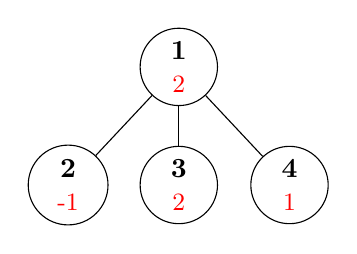
\begin{tikzpicture}[sibling distance=4em, every node/.style = {shape=circle,
	draw, align=center, top color=white, bottom color=white}]]

	\node {\textbf{1} \\{\small \color{red}2}}
	child { node {\textbf{2} \\{\small \color{red}-1}} }
	child { node {\textbf{3} \\{\small \color{red}2}} }
	child { node {\textbf{4} \\{\small \color{red}1}} };
	\end{tikzpicture}
\end{center}
We pick vertices $3$ and $4$ for a total weight of $2+1=3$.

\subsection*{Sample 2}
\begin{tabular}{p{0.5\textwidth} p{0.3\textwidth}}
	\textbf{Input} & \textbf{Output} \\
	\hline
	\begin{minted}{text}
10
15 8 8 -4 15 14 12 14 11 11
7 1
1 2
7 3
1 4
7 5
7 6
2 8
10 9
1 10
	\end{minted}
	&
	\begin{minted}{text}
77
	\end{minted}
\end{tabular}

\begin{center}
	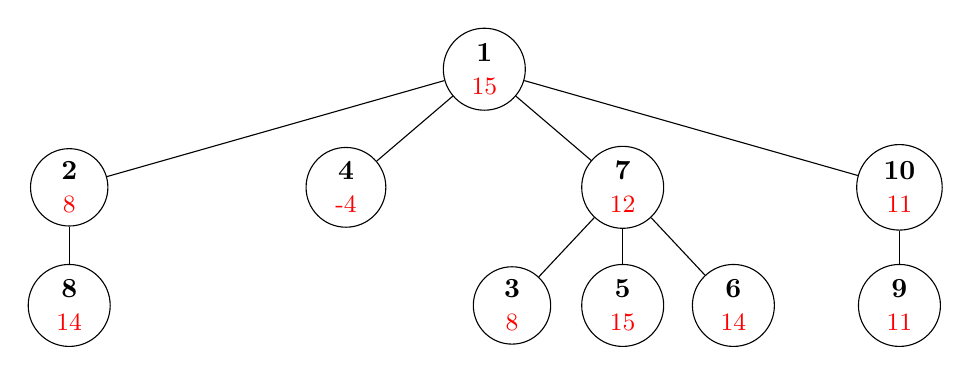
\begin{tikzpicture}[ 
		level 1/.style={sibling distance=10em},
		level 2/.style={sibling distance=4em},
		level 3/.style={sibling distance=0em},
		every node/.style = {shape=circle,
		draw, align=center, top color=white, bottom color=white}]]

	\node {\textbf{1} \\{\small \color{red}15}}
	child { node {\textbf{2} \\{\small \color{red}8}} 
		child { node {\textbf{8} \\{\small \color{red}14}} }
	}
	child { node {\textbf{4} \\{\small \color{red}-4}} }
	child { node {\textbf{7} \\{\small \color{red}12}} 
		child { node {\textbf{3} \\{\small \color{red}8}} }
		child { node {\textbf{5} \\{\small \color{red}15}} }
		child { node {\textbf{6} \\{\small \color{red}14}} }
	}
	child { node {\textbf{10} \\{\small \color{red}11}}
		child { node {\textbf{9} \\{\small \color{red}11}} }
	};
	\end{tikzpicture}
\end{center}
We pick vertices 1, 3, 5, 6, 8, 9 with a total value of $77$.

\thispagestyle{empty}

\end{document}
